% \documentclass[12pt,a4paper]{scrartcl}
\documentclass[12pt,letterpaper]{scrartcl}
\usepackage{amsmath,amsthm,amssymb,graphicx,setspace,natbib,dcolumn,float,booktabs,bm,footmisc,url,longtable,lscape,titling,hyperref,newtxtext}
\usepackage[top=1in,bottom=1in,outer=1in,inner=1in]{geometry}
\usepackage[justification=raggedright,labelsep=period,labelfont=bf,singlelinecheck=off]{caption}
\usepackage[normalem]{ulem}
\usepackage[nottoc,notlot,notlof]{tocbibind}
\urlstyle{same}
\bibpunct[, ]{(}{)}{;}{a}{}{,}
\newcolumntype{a}{D{.}{.}{0}}
\newcolumntype{b}{D{.}{.}{2}}
\newcolumntype{d}{D{.}{.}{3}}
\newcolumntype{,}{D{,}{,}{-1}}
\setlength{\footnotesep}{\baselineskip}
\let\footnotesize\normalsize
\let\oldfootnote\footnote
\renewcommand\footnote[1]{\oldfootnote{\hspace{2mm}#1}}
\setlength{\bibsep}{0pt}
\renewcommand\bibname{References}
\renewcommand{\thefigure}{A.\arabic{figure}}
\renewcommand{\thetable}{A.\arabic{table}}
\renewcommand{\theequation}{A.\arabic{equation}}
\renewcommand{\footnotelayout}{\doublespacing}
\renewcommand{\thesection}{\Alph{section}}
\renewcommand{\topfraction}{1.0}
\renewcommand{\textfraction}{0.01}

% == Cross Referencing Different Docs
\usepackage{xr}
\externaldocument{maintext_POQ}

% the following script is needed to reference appendix in the main text when using overleaf
\makeatletter
\newcommand*{\addFileDependency}[1]{% argument=file name and extension
\typeout{(#1)}% latexmk will find this if $recorder=0
% however, in that case, it will ignore #1 if it is a .aux or
% .pdf file etc and it exists! If it doesn't exist, it will appear
% in the list of dependents regardless)
%
% Write the following if you want it to appear in \listfiles
% --- although not really necessary and latexmk doesn't use this
%
\@addtofilelist{#1}
%
% latexmk will find this message if #1 doesn't exist (yet)
\IfFileExists{#1}{}{\typeout{No file #1.}}
}\makeatother

\newcommand*{\myexternaldocument}[1]{%
\externaldocument{#1}%
\addFileDependency{#1.tex}%
\addFileDependency{#1.aux}%
}

% change this to 0 to show author names
\newcommand{\blind}{1}

\allowdisplaybreaks
\preauthor{}
\postauthor{}
\predate{}
\postdate{}
\title{\textbf{\textsf{\LARGE Online Appendix for\linebreak The Rally Effect Reexamined:\linebreak New Insights from Weekly Polling Data in Japan}}}
\author{
  \if0\blind
  \hspace{1.5in}
  Hirofumi Miwa\thanks{Professor, Faculty of Law, Gakushuin University,
  Tokyo, Japan. URL: \href{https://sites.google.com/site/miwahirofumi/en}{https://sites.google.com/site/miwahirofumi/en}}
  \hspace{.7in}
  Tomoya Sasaki\thanks{Ph.D. Candidate, Department of
  Political Science, Massachusetts Institute of Technology,
  Cambridge, MA, 02139. Email:
  \href{mailto:tomoyas@mit.edu}{tomoyas@mit.edu},
  URL: \href{https://tomoya-sasaki.github.io/}{https://tomoya-sasaki.github.io/}}
  % \hspace{.7in}
  \fi
}
\date{}

\begin{document}

\begin{titlepage}
\maketitle
\setcounter{tocdepth}{2}
\tableofcontents
\thispagestyle{empty}
\end{titlepage}

\defcitealias{CSIS2023}{CSIS}
\defcitealias{PCIA2023}{PCIA}
\defcitealias{START2022}{START}

\normalsize
\doublespacing
\section{Related Literature}\label{app:sec:literature}

\subsection{\citet{seo2023}}\label{app:subsec:seo2023}

This section presents the difference between our work and that of \citet{seo2023}, which has recently offered one of the most rigorous empirical analyses on the ``rally 'round the flag'' effect. We also point out potential limitations of their analysis.

\citet{seo2023} study the rally effect for militarized interstate disputes (MID) using multiple waves of worldwide Gallup surveys. Their goal is to causally identify the rally effect by analyzing the effect of MIDs that occurred in the middle of the survey and comparing the survey responses before and after each of these MIDs. They report that MIDs do not increase but instead decrease support for national leaders, which contradicts with a prediction of the ``rally 'round the flag'' phenomena.

Although they provide a comprehensive analysis that challenges the ``rally 'round the flag'' phenomena, their study has several limitations. First, their analysis does not necessarily account for deliberate choices to participate in MIDs. As they admit, since leaders make strategic decisions to engage in MIDs, the negative effect might be driven by the scenario where a leader strategically initiates an MID or provokes another country to counteract unfavorable domestic conditions happening simultaneously and divert public attention. Therefore, their findings may not properly capture the rally effect due to the potential for diversionary foreign policy. We focus on Japan to mitigate this concern. As discussed, Japan is an ideal case to study the rally effect as the Constitution does not permit the Japanese government to initiate any provocative action and therefore we can treat external threats as exogenous to leader's incentives.

Second, their results do not necessarily hold once we properly account for the uncertainty of the estimates, potentially altering the implications of their conclusions. \citet{seo2023} report heteroskedasticity robust standard errors without any clustering. We argue that clustering the standard errors of the regression coefficients at the MID level is a necessary step to account for the uncertainty of the estimated coefficients adequately since it is highly likely that responses from survey participants who are exposed to the same MID are correlated with each other. Moreover, survey participants exposed to the same MID are in the same wave of Gallup surveys, which gives another reason to believe that their responses are not independent within each wave. For these reasons, in our replication exercise below, we cluster the standard errors of the regression coefficients at the MID level (i.e., survey-wave level), leaving all other aspects of the original study unchanged.

Figure~\ref{app:fig:replication} displays the replication of the main analysis in \citet{seo2023} and our additional analysis where the standard errors of the corresponding coefficients are clustered at each MID.\footnote{Replication materials of \citet{seo2023} are available at \href{https://dataverse.harvard.edu/dataset.xhtml?persistentId=doi:10.7910/DVN/SM6MZM}{https://dataverse.harvard.edu/dataset.xhtml?persistentId=doi:10.7910/DVN/SM6MZM}.} The dots indicate the average treatment effects and the vertical lines show their corresponding 95\% confidence intervals. The circle and triangle dots represent the original and our additional results, respectively. The outcome of interest is the public approval of a political leader's job performance.

As Figure~\ref{app:fig:replication} shows, the original study finds that the onset of MID decreases (increases) the approval (disapproval) of the job performance with high confidence. Based on these findings, \citet{seo2023} concludes that they do not find evidence of the rally effect. However, our additional analysis, where we cluster the standard errors of the regression coefficients at the MID level, shows that the standard errors of the coefficients are much larger than the original results, and the 95\% confidence intervals always include zero. These results suggest that we cannot necessarily conclude that the onset of MID decreases (increases) the approval (disapproval) of the job performance. Again, the only difference between their approaches and ours is how to account for uncertainty. Therefore, the original results are not robust to the clustering of the standard errors at the MID level, and they do not provide strong evidence against the rally effect.

\begin{figure}[!ht]
  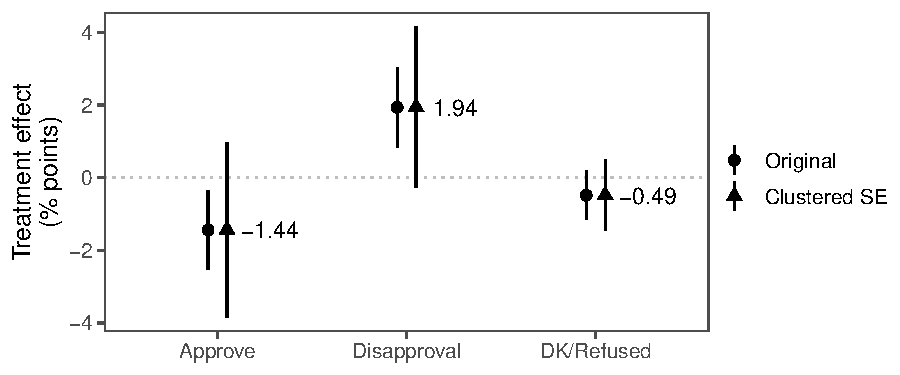
\includegraphics[width = \linewidth]{Figure_POQ/Figure_1_revised.pdf}
  \caption{Replication of Figure~1 of \citet{seo2023}. The original results do not cluster the standard errors of the coefficient, whereas in our replication results labeled as ``Clustered SE,'' we cluster the standard errors at the MID level.}\label{app:fig:replication}
\end{figure}

Apart from the points discussed above, our study is also different from \citet{seo2023} in two significant ways. First, we include terrorism as an external threat, which is omitted from their work. Second, we estimate the duration of the rally effect.

\subsection{Studying Rally Effect in Japan}\label{app:subsec:rally_japan}

Several previous studies have examined the rally 'round the flag phenomenon in Japan. This section reviews these studies and describes our contribution distinct from them.

There are two studies using aggregate time-series data of Cabinet approval, but the results are mixed. \citet{kagotani2015} uses monthly public opinion data and pooling MID incidents around Japan to explore the rally effect from 1990 to 2004 (that is, after the Cold War). This work finds that the foreign threats increase Cabinet approval. In contrast, \citet{Ohmura2014Leviathan} use the same opinion poll and MID data as \citet{kagotani2015} but reveal that, while MIDs caused the rally effect during the Cold War, this is not the case in the post-Cold War period. We speculate that these non-robust outcomes may be attributable to too coarse‐grained time series.

Several other studies explicate the microfoundation of the rally effects using survey experiments, which overcomes the problem caused by the coarseness of data points. \citet{kobayashi2018} find that exposure to news on the Senkaku Island dispute raised participants' anger toward China but did not necessarily increase public support for the prime minister. Because they used an experimental design, their focus is restricted to a particular dispute, thereby limiting the external validity of their findings. \citet{Hata2023} shares its interest with us in that it examines the effect of North Korean missile launches.\footnote{To be more precise, he studies the effect of alerts for the launches issued by the Japanese government.} Still, the outcome variable is an attitude toward the amendment of the Constitution's pacifist clause, not support for the government, which the literature on the rally effect has originally addressed.

A study relying on a natural experiment gets the best of both worlds of the above two approaches. \citet{fukumoto2023} employs ``unexpected events during survey'' design, as \citet{seo2023} do, to identify an indirect rally effect where wars involving third-party countries increase the popularity of the ruling party. Their research shares our interest in examining the effects of terrorist attacks abroad in that it focuses on international events not directly related to Japan, but its outcome is people's support for the ruling party, not government popularity per~se.

In contrast to these studies, we comprehensively investigate the rally effect for various types of events, utilizing government popularity data with time scales shorter than monthly intervals.

\section{Additional Information on Empirical Strategy}\label{app:sec:japan}

As discussed in the main text, we leverage Japan's pacifist Constitution to treat North Korea's military threats and foreign terrorism as exogenous, as Japan cannot initiate military provocations. Furthermore, Japan's pacifist Constitution prohibits its government from engaging in military reactions against North Korea or terrorist groups.

We provide further discussion about our empirical strategy. First, there is a consensus among experts that Japanese government and public have adopted very restrained attitudes towards potential adversaries.\footnote{\href{https://www.armscontrol.org/act/2007-06/features/not-going-nuclear-japans-response-north-koreas-nuclear-test}{https://www.armscontrol.org/act/2007-06/features/not-going-nuclear-japans-response-north-koreas-nuclear-test}; accessed January 20th, 2024.} Japan has strengthened its ties with the U.S. primarily to deter North Korea and China, but it does not lead to the heightened immediate military reactions against each of North Korea's military tests or terrorism \citep{izumi2007,izumikawa2017}. Second, following the Constitution, Japan does not possess military capabilities to conduct initial attacks against potential adversaries during our period of analysis.\footnote{\url{https://carnegieendowment.org/programs/asia/japan-military-strike-debate/}; accessed January 20th, 2024} Although acquiring counter strike capability or enemy base strike capability (\textit{teki kichi kogeki noryoku}) had been debated since 1960s and the government decided to acquire the missile strike capability in 2026, Japanese government does not have the means to initiate military provocations.

\section{Additional Information on Data}\label{app:sec:data}


\subsection{List of Rally Events}\label{app:subsec:events}


Tables~\ref{list_missile_launchings}--\ref{list_other_terrorism} list the incidents coded as missile launches, nuclear tests, Japanese-targeted terrorism, and other terrorism in this study. Because we code the dates of Japanese-targeted terrorism and other terrorism as the day on which \emph{Asahi Shimbun} reported it in Japan, dates in the lists do not necessarily coincide with the dates when the incidents occurred in local time.

\small
\singlespacing
\begin{longtable}[c]{lll}
\caption{\normalsize{List of Missile and Satellite Launches by North Korea}}
\label{list_missile_launchings}
\bigskip \\\toprule
\multicolumn{1}{c}{Date} & \multicolumn{1}{c}{Day} & \multicolumn{1}{c}{Event} \\\midrule
\endfirsthead
\caption{\normalsize{List of Missile and Satellite Launches by North Korea (continued)}}
\bigskip \\\toprule
\multicolumn{1}{c}{Date} & \multicolumn{1}{c}{Day} & \multicolumn{1}{c}{Event} \\\midrule
\endhead
\bottomrule
\endfoot
May 1, 2005 & Sun & Anti-ship cruise missile \\
Jul 4, 2006 & Thu & Inter-continental ballistic missile/short-range missile launches. \\
Apr 5, 2009 & Sun & Satellite (other provocation) \\
Jul 4, 2009 & Sat & Medium-range ballistic missile \\
Apr 13, 2012 & Fri & Satellite (other provocation) \\
Dec 12, 2012 & Wed & Satellite (other provocation) \\
Mar 26, 2014 & Wed & Medium-range ballistic missile \\
Jun 29, 2014 & Sun & Short-range ballistic missile \\
Feb 7, 2016 & Sun & Satellite (other provocation) \\
Apr 23, 2016 & Sat & Ballistic missile from submarine \\
Jun 22, 2016 & Wed & Intermediate-range ballistic missile \\
Aug 3, 2016 & Wed & Medium-range ballistic missile \\
Aug 24, 2016 & Wed & Ballistic missile from submarine \\
Sep 5, 2016 & Mon & Medium-range ballistic missile \\
Mar 6, 2017 & Mon & Medium-range ballistic missile \\
Apr 5, 2017 & Wed & Short-to-medium-range ballistic missile \\
Apr 16, 2017 & Sun & Ballistic missile (unknown type) \\
Apr 29, 2017 & Sat & Short-to-medium-range ballistic missile \\
May 14, 2017 & Sun & Intermediate-range ballistic missile \\
May 21, 2017 & Sun & Medium-range ballistic missile \\
May 29, 2017 & Mon & Short-range ballistic missile \\
Jul 4, 2017 & Tue & Inter-continental ballistic missile \\
Jul 28, 2017 & Fri & Inter-continental ballistic missile \\
Aug 29, 2017 & Tue & Ballistic missile (unknown type) \\
Sep 15, 2017 & Fri & Intermediate-range ballistic missile \\
Nov 29, 2017 & Wed & Inter-continental ballistic missile \\
May 4, 2019 & Sat & Short-range ballistic missile \\
May 9, 2019 & Thu & Short-range ballistic missile \\
Jul 25, 2019 & Thu & Short-range ballistic missile \\
Aug 24, 2019 & Sat & Short-range missile \\
Oct 2, 2019 & Wed & Short-range missile \\
Mar 25, 2021 & Thu & Short-range missile \\
Sep 15, 2021 & Wed & Short-range missile \\
Sep 28, 2021 & Tue & Short-range missile \\
Jan 30, 2022 & Sun & Intermediate-range ballistic missile \\
Mar 24, 2022 & Thu & Intercontinental ballistic missile \\
Jun 5, 2022 & Sun & Short-range ballistic missile \\
Oct 4, 2022 & Tue & Intermediate-range ballistic missile \\
Oct 6, 2022 & Thu & Short-range ballistic missile \\
Nov 2, 2022 & Wed & Short-range ballistic missile \\
Nov 3, 2022 & Thu & Intercontinental and short-range ballistic missiles \\
Nov 5, 2022 & Sat & Short-range ballistic missile \\
Nov 18, 2022 & Fri & Intercontinental ballistic missile \\
Feb 18, 2023 & Sat & Intercontinental ballistic missile \\
Mar 16, 2023 & Thu & Intercontinental ballistic missile \\
Apr 13, 2023 & Thu & ballistic missile (type unknown) \\
May 30, 2023 & Tue & Satellite \\
Jun 15, 2023 & Thu & Short-range ballistic missile \\
\end{longtable}

\small
\noindent \emph{Notes}: Data sourced from \citetalias{CSIS2023} \citeyearpar{CSIS2023}.

\begin{table}[H]
\begin{minipage}{\hsize}
\centering
\small
\singlespacing
\caption{Dates of Nuclear Tests by North Korea}
\label{list_nuclear_tests}
\bigskip
\begin{tabular}{lll}\toprule
\multicolumn{1}{c}{Date} & \multicolumn{1}{c}{Day} & \multicolumn{1}{c}{Event} \\\midrule
Oct 9, 2006 & Mon & Nuclear test \\
May 25, 2009 & Mon & Nuclear test \\
Feb 12, 2013 & Thu & Nuclear test \\
Jan 6, 2016 & Wed & Nuclear test \\
Sep 9, 2016 & Fri & Nuclear test \\
Sep 3, 2017 & Sun & Nuclear test \\\bottomrule
\end{tabular}
\end{minipage}
\begin{minipage}{\hsize}
\bigskip
\small
\singlespacing
\emph{Notes}: Data sourced from \citetalias{CSIS2023} \citeyearpar{CSIS2023}.
\end{minipage}
\end{table}

\begin{table}[H]
\begin{minipage}{\hsize}
\centering
\small
\singlespacing
\caption{List of Japanese-Targeted Terrorism}
\label{list_Japanese_targeted_terrorism}
\bigskip
\begin{tabular}{llll}\toprule
\multicolumn{1}{c}{Date} & \multicolumn{1}{c}{Day}& \multicolumn{1}{c}{Country} & \multicolumn{1}{c}{Event} \\\midrule
Dec 1, 2003 & Mon & Iraq & Two diplomats were killed. \\
Apr 9, 2004 & Fri & Iraq & Three citizens were kidnapped. \\
Apr 15, 2004 & Thu & Iraq & Two journalists were kidnapped. \\
May 29, 2004 & Sat & Iraq & Two journalists were killed. \\
Oct 28, 2004 & Thu & Iraq & A tourist was kidnapped (subsequently killed). \\
May 10, 2005 & Tue & Iraq & A security company employee was taken into custody \\
 & & & (subsequently killed). \\
Aug 27, 2008 & Wed & Afghanistan & An NGO member was kidnapped (subsequently killed). \\
Apr 3, 2010 & Sat & Afghanistan & A journalist was kidnapped. \\
Aug 21, 2012 & Tue & Syria & A journalist was killed. \\
Jan 21, 2015 & Wed & Syria & A businessperson and a journalist were kidnapped \\
 & & & (subsequently killed). \\
Oct 4, 2015 & Sun & Bangladesh & A farmer was killed. \\\bottomrule
\end{tabular}
\end{minipage}
\centering
\begin{minipage}{\hsize}
\bigskip
\small
\singlespacing
\emph{Notes}: Data sourced from the \citetalias{PCIA2023} \citeyearpar{PCIA2023} list of ``major terrorism incidents that harmed Japanese.'' NGO = non-governmental organization.
\end{minipage}
\end{table}

\small
\singlespacing
\begin{longtable}[c]{lllllr}
\caption{\normalsize{List of Other Terrorism}}
\label{list_other_terrorism}
\bigskip \\\toprule
\multicolumn{1}{c}{Date} & \multicolumn{1}{c}{Day}& \multicolumn{1}{c}{Country} & \multicolumn{1}{c}{City} & \multicolumn{1}{c}{Event} \\\midrule
\endfirsthead
\caption{\normalsize{List of Other Terrorism (continued)}}
\bigskip \\\toprule
\multicolumn{1}{c}{Date} & \multicolumn{1}{c}{Day}& \multicolumn{1}{c}{Country} & \multicolumn{1}{c}{City} & \multicolumn{1}{c}{Event} \\\midrule
\endhead
\bottomrule
\endfoot
Sep 12, 2001 & Wed & U.S. & New York, etc. & The 9/11 attack \\
Oct 29, 2001 & Mon & Philippines & Zamboanga City & Bombings at a downtown area \\
Oct 14, 2002 & Mon & Indonesia & Kuta & 2002 Bali bombings \\
Oct 18, 2002 & Fri & Philippines & Zamboanga, etc. & Bombings at a department store, etc. \\
Oct 25, 2002 & Fri & Russia & Moscow & Moscow theater hostage crisis \\
Mar 5, 2003 & Wed & Philippines & Davao & Bombing at an airport \\
Jul 6, 2003 & Sun & Russia & Pokrovskoye- & Bombings at a rock festival \\
 & & & \hspace{0.5em}Streshnevo & \\
Aug 6, 2003 & Wed & Indonesia & Jakarta & Bombing at a hotel \\
Dec 6, 2003 & Sat & Russia & Yessentuki & Bombing in a train \\
Feb 7, 2004 & Sat & Russia & Zamoskvorechye & Bombing in a subway train \\
Mar 12, 2004 & Fri & Spain & Madrid & 2004 Madrid train bombings \\
Aug 26, 2004 & Thu & Russia & Rostov-on-Don & 2004 Russian aircraft bombings \\
 & & & \hspace{0.5em}and Gluboky & \\
Sep 2, 2004 & Thu & Russia & Beslan & Beslan school hostage crisis \\
Jul 8, 2005 & Fri & U.K. & London & 7 Jul 2005 London bombings \\
Oct 2, 2005 & Sun & Indonesia & Jimbaran & 2005 Bali bombings \\
Jul 22, 2008 & Tue & China & Kunming & Bombings in buses \\
Nov 28, 2008 & Fri & India & Mumbai & 2008 Mumbai attacks \\
Mar 30, 2010 & Tue & Russia & Moscow & Bombings at subway stations \\
Jan 25, 2011 & Tue & Russia & Domodedovo & Bombing at an airport \\
Jul 23, 2011 & Sat & Norway & Oslo & 2011 Norway attacks \\
Jan 17, 2013 & Thu & Algeria & In Amenas & In Amenas hostage crisis \\
Apr 16, 2013 & Tue & U.S. & Boston & Boston Marathon bombing \\
Oct 29, 2013 & Tue & China & Beijing & 2013 Tiananmen Square attack \\
Dec 30, 2013 & Mon & Russia & Volgograd & Bobmings at a station \\
Dec 31, 2013 & Tue & Russia & Volgograd & Bobmings in a bus \\
May 1, 2014 & Thu & China & Urumqi & Bobming at a station \\
May 23, 2014 & Fri & China & Urumqi & Car attack and bombings at a market \\
Jan 8, 2015 & Thu & France & Paris & \emph{Charlie Hebdo} shooting \\
Feb 16, 2015 & Mon & Denmark & Copenhagen & Shootings at a cultural center, etc. \\
Mar 19, 2015 & Thu & Tunisia & Tunis & Bardo National Museum attack \\
Jun 27, 2015 & Sat & France & Saint-Quentin- & Car attack an air products factory \\
 & & & \hspace{0.5em}Fallavier & \\
Aug 18, 2015 & Tue & Thailand & Bangkok & 2015 Bangkok bombing \\
Nov 15, 2015 & Sun & France & Paris & Nov 2015 Paris attacks \\
Dec 4, 2015 & Fri & U.S. & San Bernardino & 2015 San Bernardino attack \\
Jan 15, 2016 & Fri & Indonesia & Jakarta & Bombings at a cafe, etc. \\
Mar 23, 2016 & Wed & Belgium & Brussels & 2016 Brussels bombings \\
Jun 13, 2016 & Mon & U.S. & Orlando & Orlando nightclub shooting \\
Jul 3, 2016 & Sun & Bangladesh & Dhaka & Jul 2016 Dhaka attack \\
Jul 9, 2016 & Sat & U.S. & Dallas & Shooting of police officers \\
Jul 15, 2016 & Fri & France & Nice & 2016 Nice attack \\
Jul 23, 2016 & Sat & Germany & Munich & Shooting at a shopping mall \\
Dec 20, 2016 & Tue & Germany & Berlin & 2016 Berlin attack \\
Mar 23, 2017 & Thu & U.K. & London & 2017 Westminster attack \\
Apr 4, 2017 & Tue & Russia & Saint & 2017 Saint Petersburg Metro bombing \\
 & & & \hspace{0.5em}Petersburg & \\
Apr 21, 2017 & Fri & France  & Paris  & Shooting of police officers \\
May 23, 2017 & Tue & U.K. & Manchester & Manchester Arena bombing \\
Jun 5, 2017 & Mon & U.K. & London & Jun 2017 London Bridge attack \\
Aug 18, 2017 & Fri & Spain & Barcelona & 2017 Barcelona attacks \\
Oct 3, 2017 & Tue & U.S. & Las Vegas & 2017 Las Vegas shooting \\
Nov 2, 2017 & Thu & U.S. & New York & 2017 New York City truck attack \\
May 14, 2018 & Mon & France & Paris & 2018 Paris knife attack \\
May 14, 2018 & Mon & Indonesia & Surabaya & Bombings at churches \\
Oct 28, 2018 & Sun & U.S. & Pittsburgh & Pittsburgh synagogue shooting \\
Mar 16, 2019 & Sat & New Zealand & Christchurch & Christchurch mosque shootings \\
Apr 22, 2019 & Mon & Sri Lanka & Colombo, etc. & 2019 Sri Lanka Easter bombings \\
Oct 17, 2020 & Sat & France & Paris & Murder of Samuel Paty \\
Nov 4, 2020 & Wed & Austria & Vienna & 2020 Vienna attack \\
\end{longtable}

\noindent \emph{Notes}: Data sourced from \emph{Asahi Shimbun} and \citetalias{START2022} \citeyearpar{START2022} (the latter covers events only in 2020 or earlier).

% \subsection{Outcome Variables}\label{app:subsec:outcome}

% The government popularity is typically measured using the following question: ``Do you support the cabinet of [prime minister's surname]?'' and party support is usually measured with the following question: ``Which party do you support?''

\normalsize
\doublespacing
\subsection{Additional Information on Explanatory Variables}\label{app:subsec:terrorism}

This study focuses on the effects of events abroad on the government's popularity. Except for the two events mentioned below, no terrorist incidents with fatalities occurred in Japan during the period of our analysis. We add notes on the two exceptions here.

In the Global Terrorism Database of the version we used, which covers December 31, 2021 or earlier, there is one recorded incident in Japan in which at least one fatality occurred, excluding that of the perpetrator. This was a stabbing attack at a residential care center in Sagamihara, Kanagawa Prefecture, on July 26, 2016, in which one assailant killed 19 mentally handicapped persons. Although this incident had a great impact on Japanese society, we do not treat it as Japanese-targeted terrorism not only because it was a domestic event but also because major newspapers did not report this stabbing as a terrorist attack. \citet{Huff2018AJPS} contended that whether citizens perceive a violent act as terrorism is greatly affected by media framing. Moreover, the defendant in this case had a history of mental illness, which is one of the factors that lowers the likelihood of citizens perceiving an incident as terrorism \citep{Huff2018AJPS}.

After the period covered by the Global Terrorism Database, the former prime minister Shinzo Abe was assassinated. This assassination was definitely recognized as a terrorist incident by the Japanese people. Nonetheless, we exclude this event from our analysis because of its distinct nature compared to other events, thereby clarifying the scope of our study. The fluctuation in Cabinet approval that might be caused by this assassination should be absorbed as a random error in the autoregressive process of the transition model in our ``pooling the polls'' analysis.

\subsection{Additional Information on Control Variables}\label{app:subsec:control}

This section offers detailed information on control variables. We include the scandals related to cabinet members detailed in chapter~4 of \citet{Carlson2018} as ministerial scandals. Because \citet{Carlson2018} do not cover the period after 2016, scandals in the later period are identified by the authors. We add all scandals that eventually led to the resignation of ministers to the list. Moreover, we also consider the Moritomo scandal and the Kake scandal, which are related to the former prime minister Shinzo Abe and hugely degraded the Cabinet. The date of each scandal is recorded as that on which it was first reported in major newspapers. Ministerial resignation includes cases in which the prime minister fired a minister and a ministerial suicide. For election results, we code LDP victories in 2001, 2005, 2010, 2012, 2013, 2014, 2016, and 2017; DPJ victories are coded in 2003, 2004, 2007, and 2009. Closing of the Diet equals 1 if a session longer than one month is closed in that week and 0 otherwise. Because controversial bills are usually passed at the end of sessions, the cabinet approval rating is expected to decrease, on average, in the week in which a session closes.

\section{Details on Parameter Estimation}\label{app:sec:estimation}

\subsection{Statistical Software and Packages}

This study's analysis was conducted by R~4.2.3 \citep{R2023}. We used JAGS~4.3.0 \citep{Plummer2017} and \texttt{runjags} package version 2.2.1--7 \citep{Denwood2016JStatSoftware} to perform MCMC sampling, and \texttt{coda} package version 0.19--4 \citep{Plummer2006RNews} to postprocess MCMC outputs.

\subsection{MCMC Procedure}\label{app:subsec:mcmc}

For all prime ministers, we set the prior distributions of the approval ratings in the first week as $\alpha _{1}\sim \mathrm{U}(l_{0},u_{0})$, where $l_{0}$ and $u_{0}$ are plus and minus 20 percentage points of the rating measured by the first poll taken by \emph{Asahi Shimbun} during the period. Moreover, we assume that the prior distributions of $\omega $, $\nu _{j}$, and $\tau _{ks}$ are $\mathrm{U}(0,100)$, and that of the remaining parameters are $\mathrm{N}(0,100^{2})$. We set three chains and inputted different sets of initial values. For each chain, we obtained 10,000 samples at every 10th interval after an adaptation period of 1,000 and a burn-in period of another 1,000. Based on the Gelman-Rubin statistics, we judged that all the chains converged.

\section{Additional Information for Main Results}\label{app:sec:misc_cabinet}

The top panel of Figure~\ref{approval_time_series} shows the weekly cabinet approval ratings estimated by the models without interaction terms between events and their temporal distance to opinion polls (Equation~\eqref{transition_model} in the main text). Solid lines represent point estimates, and shaded areas represent 95\% credible intervals (CIs). The estimation results of house, mode, and design effects are shown in Figure~\ref{house_mode_design_cabinet}. Dots represent point estimates, and lines represent 95\% CIs. The estimation results of other miscellaneous parameters are shown in Table~\ref{miscellaneous_cabinet}. Table~\ref{table_eta_cabinet} shows the estimated coefficients of control variables in the transition model with interaction terms between events and their temporal distance to opinion polls (i.e., Equation~\eqref{transition_model_2} in the main text).

\begin{table}[H]
\centering
\small
\singlespacing
\caption{Estimates of $\bm{\eta }$ in the Transition Model for Cabinet Approval Ratings with Interaction Terms between Events and their Temporal Distance to Opinion Polls}
\label{table_eta_cabinet}
\bigskip
\begin{tabular}{ld,}\toprule
 & \multicolumn{1}{c}{Point est.} & \multicolumn{1}{c}{95\% CI} \\\midrule
Cabinet reshuffle & 0.031 & [0.015,\: 0.048] \\
Ministerial scandal & -0.007 & [-0.020,\: 0.007] \\
Ministerial resignation & -0.006 & [-0.020,\: 0.008] \\
Incumbent party victory & 0.033 & [0.010,\: 0.055] \\
Incumbent party defeat & -0.040 & [-0.080,\: 0.000] \\
Closing of the Diet & -0.013 & [-0.023,\: -0.003] \\
$\Delta $~Nikkei~225 / 1000 & 0.002 & [-0.002,\: 0.006] \\\bottomrule
\end{tabular}
\end{table}

\begin{landscape}
\begin{figure}[t]
\begin{minipage}{\hsize}
\centering
\singlespacing
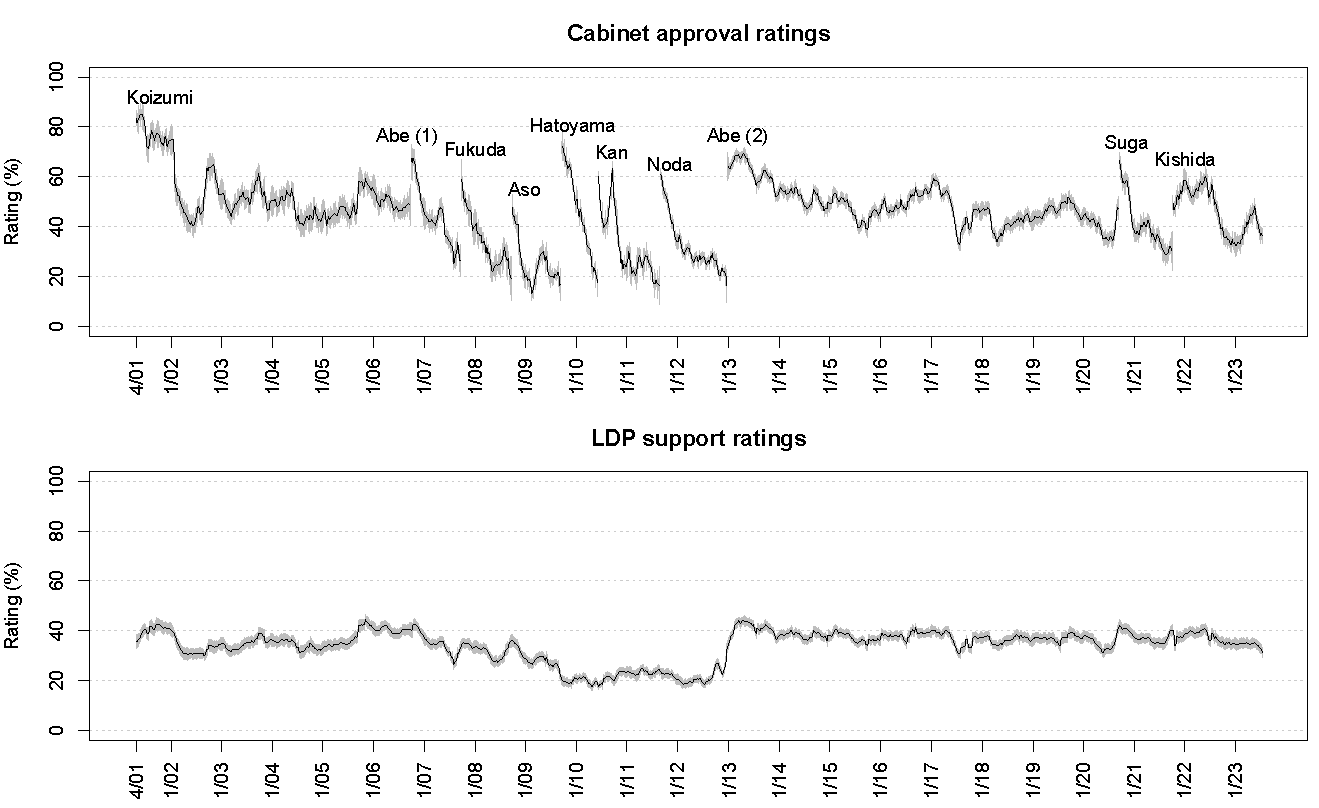
\includegraphics[scale=1]{Figure_POQ/approval_time_series.pdf}
\caption{Estimated Weekly Cabinet Approval and LDP Support Ratings}
\label{approval_time_series}
\end{minipage}
\begin{minipage}{\hsize}
\bigskip
\small
\emph{Notes}: Solid lines represent point estimates, and shaded areas represent 95\% CIs.
\end{minipage}
\end{figure}
\end{landscape}

\begin{figure}[p]
\begin{minipage}{\hsize}
\centering
\singlespacing
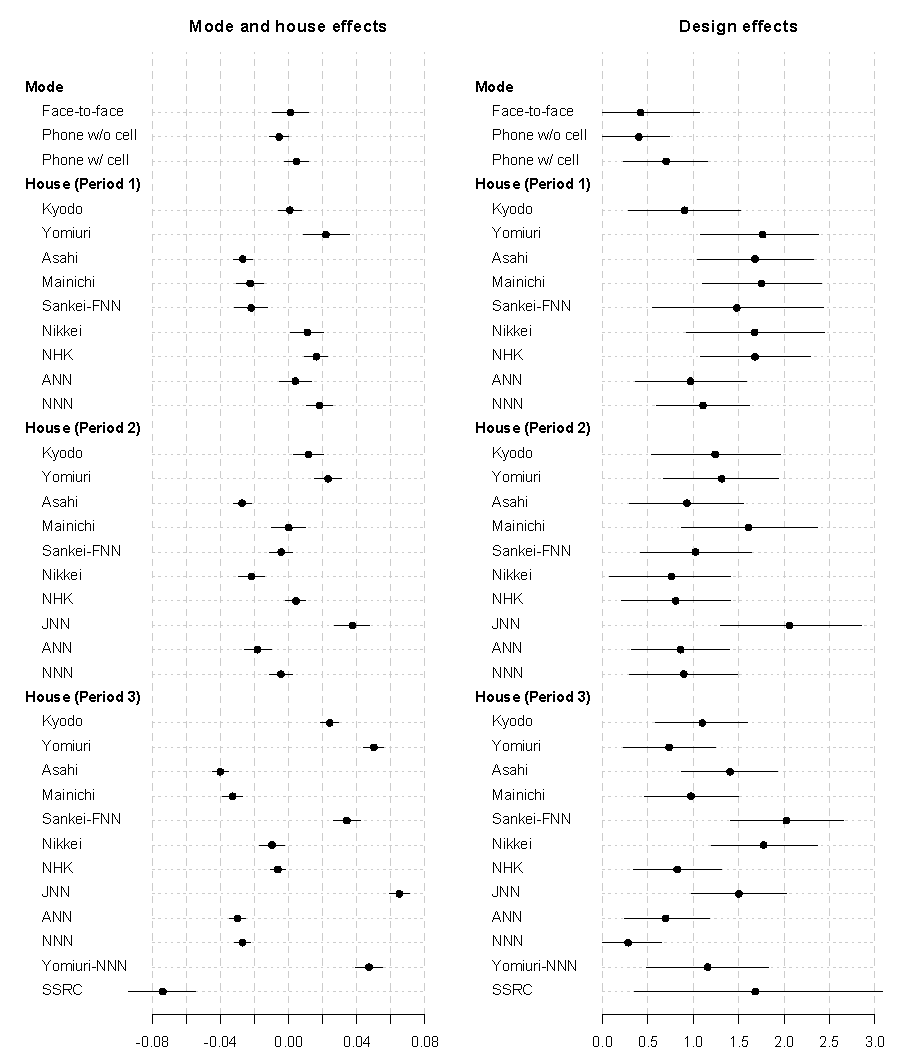
\includegraphics[scale=1]{Figure_POQ/miscellaneous_cabinet_approval.pdf}
\caption{Estimation Results of House, Mode, and Design Effects for Cabinet Approval Ratings}
\label{house_mode_design_cabinet}
\end{minipage}
\begin{minipage}{\hsize}
\singlespacing
\small
\emph{Notes}: Dots represent point estimates, and lines represent 95\% CIs.
\end{minipage}
\end{figure}

\begin{table}[p]
\centering
\small
\singlespacing
\caption{Estimation Results of Miscellaneous Parameters for Cabinet Approval Ratings}
\label{miscellaneous_cabinet}
\bigskip
\begin{tabular}{lld,}\toprule
 & & \multicolumn{1}{c}{Point est.} & \multicolumn{1}{c}{95\% CI} \\\midrule
$\beta $ & Koizumi & 0.000 & [0.000,\: 0.000] \\
 & Abe (1) & -0.001 & [-0.003,\: 0.000] \\
 & Fukuda & -0.002 & [-0.004,\: 0.000] \\
 & Aso & 0.000 & [-0.001,\: 0.001] \\
 & Hatoyama & -0.013 & [-0.023,\: -0.004] \\
 & Kan & -0.001 & [-0.002,\: 0.000] \\
 & Noda & 0.000 & [-0.001,\: 0.000] \\
 & Abe (2) & 0.000 & [0.000,\: 0.000] \\
 & Suga & -0.001 & [-0.002,\: 0.001] \\
 & Kishida & 0.000 & [-0.001,\: 0.000] \\
$\psi $ & Koizumi & 0.033 & [0.008,\: 0.059] \\
 & Abe (1) & 0.117 & [0.015,\: 0.232] \\
 & Fukuda & 0.146 & [0.016,\: 0.293] \\
 & Aso & 0.028 & [-0.015,\: 0.072] \\
 & Hatoyama & 0.623 & [0.191,\: 1.098] \\
 & Kan & 0.075 & [0.007,\: 0.142] \\
 & Noda & 0.033 & [-0.011,\: 0.077] \\
 & Abe (2) & 0.019 & [0.000,\: 0.038] \\
 & Suga & 0.073 & [-0.016,\: 0.171] \\
 & Kishida & 0.051 & [0.002,\: 0.102] \\
$\phi $ & Koizumi & 0.942 & [0.902,\: 0.980] \\
 & Abe (1) & 0.788 & [0.602,\: 0.948] \\
 & Fukuda & 0.685 & [0.403,\: 0.948] \\
 & Aso & 0.870 & [0.750,\: 0.989] \\
 & Hatoyama & 0.159 & [-0.451,\: 0.730] \\
 & Kan & 0.825 & [0.691,\: 0.956] \\
 & Noda & 0.904 & [0.814,\: 0.992] \\
 & Abe (2) & 0.962 & [0.929,\: 0.993] \\
 & Suga & 0.842 & [0.664,\: 0.992] \\
 & Kishida & 0.909 & [0.823,\: 0.991] \\
$\omega $ & Koizumi & 0.028 & [0.023,\: 0.033] \\
 & Abe (1) & 0.025 & [0.015,\: 0.035] \\
 & Fukuda & 0.030 & [0.018,\: 0.043] \\
 & Aso & 0.028 & [0.020,\: 0.038] \\
 & Hatoyama & 0.023 & [0.014,\: 0.033] \\
 & Kan & 0.036 & [0.027,\: 0.045] \\
 & Noda & 0.016 & [0.011,\: 0.023] \\
 & Abe (2) & 0.017 & [0.014,\: 0.019] \\
 & Suga & 0.024 & [0.015,\: 0.034] \\
 & Kishida & 0.024 & [0.017,\: 0.031] \\\bottomrule
\end{tabular}
\end{table}

\clearpage
\section{Robustness Check}\label{app:sec:robust}

Figure~\ref{analysis_before_2017} shows the estimated average effects of military threats, terrorism, and control variables on cabinet approval ratings by the model without interaction terms using data before 2017. Some may speculate that the null result on missile launches presented in Figure~\ref{average_effect_on_cabinet_approval} of the main text is due to North Korea's escalated military provocations coinciding with scandals in the Abe Cabinet during the first half of 2017. Indeed, a quarter of missile launches analyzed herein occurred in 2017. However, even if we restrict our analysis to the period before 2017, the estimated effect of missile launches on Cabinet approval remains near zero (the point estimate is $-$0.003, and the 95\% CI is [$-$0.017, 0.011]).

\begin{figure}[!ht]
\begin{minipage}{\hsize}
\centering
\singlespacing
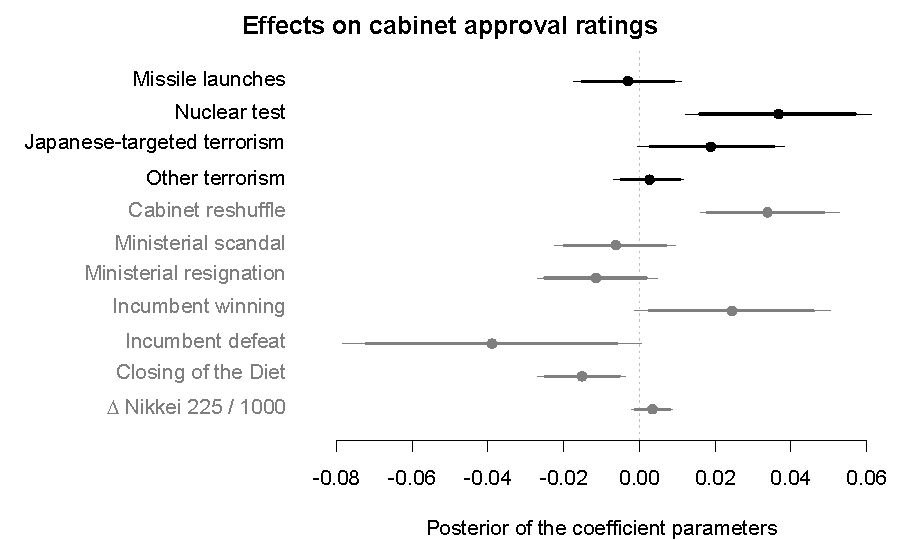
\includegraphics[scale=1]{Figure_POQ/analysis_before_2017.pdf}
\caption{Average Effects of Military Threat, Terrorism, and Other Control Variables on Cabinet Approval Ratings Using Data before 2017}
\label{analysis_before_2017}
\end{minipage}
\begin{minipage}{\hsize}
\singlespacing
\small
\emph{Notes}: Dots represent point estimates, and thick and thin lines correspond to 90\% and 95\% CIs, respectively.
\end{minipage}
\end{figure}

\section{Additional Analysis of LDP Support}\label{app:sec:res}

\subsection{Data and Variables}\label{app:subsec:ldp}

In addition to the analysis in which the outcome variable is Cabinet approval rating, we conduct an analysis where the outcome variable is the support toward the Liberal Democratic Party (LDP). The LDP is one of the two major parties in Japan during our study period and has served as a senior member of the ruling coalition. This party is noted for its hawkish stance on security and foreign issues.

Table~\ref{number_of_polls_LDP} shows the summary of polling data used in the analysis of LDP support. This table slightly differs from Table~\ref{number_of_polls} in the main text because some polls measure only either Cabinet approval or LDP support. The number of polls used here is 1,960.

\begin{table}[!b]
\begin{minipage}{\hsize}
\centering
\small
\singlespacing
\caption{Polling Result Statistics by Polling Firms and Survey Modes for the Analysis of LDP Support}
\label{number_of_polls_LDP}
\bigskip
\begin{tabular}{llaaaa}\toprule
\multicolumn{1}{c}{Polling Firm} & \multicolumn{1}{c}{Period} & \multicolumn{4}{c}{Number of Polls}\\\cmidrule{3-6}
 & & \multicolumn{1}{c}{FtF} & \multicolumn{1}{c}{Phone} & \multicolumn{1}{c}{Phone} & \multicolumn{1}{c}{Total} \\
 & & & \multicolumn{1}{c}{w/o Cell} & \multicolumn{1}{c}{w/ Cell} & \\\midrule
Kyodo Press & Jun 10, 2001--Jul 16, 2023 & 0 & 102 & 64 & 166 \\
\emph{Yomiuri Shimbun} & May 27, 2001--Jun 17, 2018 & 82 & 87 & 26 & 195 \\
\emph{Asahi Shimbun} & May 27, 2001--Jul 16, 2023 & 6 & 190 & 80 & 276 \\
\emph{Mainichi Shimbun} & Sep 2, 2001--Apr 19, 2020 & 11 & 143 & 24 & 178 \\
\emph{Sankei Shimbun}-FNN & Apr 29, 2001--Jul 16, 2023 & 0 & 132 & 31 & 163 \\
Nikkei Research & Jun 10, 2001--Jun 25, 2023 & 0 & 106 & 67 & 173 \\
NHK & May 6, 2001--Jul 9, 2023 & 0 & 173 & 68 & 241 \\
JNN & Jan 10, 2010---Jul 2, 2023 & 0 & 82 & 50 & 132 \\
ANN & Oct 29, 2006--Jul 9, 2023 & 0 & 135 & 61 & 196 \\
NNN & Dec 8, 2002--Jun 18, 2017 & 0 & 170 & 0 & 170 \\
\emph{Yomiuri Shimbun}-NNN & Jul 22, 2018--Jun 25, 2023 & 0 & 0 & 57 & 57 \\
SSRC & Apr 18, 2021--Jun 18, 2023 & 0 & 0 & 13 & 13 \\
\multicolumn{2}{l}{Total} & 99 & 1{,}320 & 541 & 1{,}960 \\\bottomrule
\end{tabular}
\end{minipage}
\begin{minipage}{\hsize}
\bigskip
\small
\emph{Notes}: This table shows polls that measure LDP support. FtF $=$ face-to-face interview; Phone w/o Cell $=$ telephone interview conducted via landline only; Phone w/ Cell $=$ telephone interview conducted via landline and cellular phones.
\bigskip

\end{minipage}
\end{table}

We use the same statistical models as in the analysis of Cabinet approval to analyze the effect of various international incidents on LDP support rates. Control variables are also largely the same. Our control variables for this analysis are \emph{cabinet reshuffle (LDP)}, \emph{LDP scandal}, \emph{ministerial resignation (LDP)}, \emph{start of an election period}, \emph{LDP victory} (national election), \emph{LDP defeat} (national election), and \emph{closing of the Diet (LDP)}, where ``(LDP)'' denotes the inclusion of only events related to the LDP government. The LDP scandals contain all ministerial scandals in the LDP government considered in the analysis of Cabinet approval. Moreover, from \citet{Carlson2018}, we include Muneo Suzuki's scandal and the Japan Dental Association's scandal, which were not related to any particular minister but greatly upset the LDP. We control for the start of an election period because it is well-known that independent voters in Japan come to state their party support when national elections are approaching \citep[e.g.,][]{Miharu2019,Nakamura2015Ehime} because some Japanese voters interpret supporting some party as an intention to vote for that party \citep{Ogura2020,Taniguchi2012}. We do not consider Nikkei~225 because it should not have affected LDP support ratings when the LDP was out of power.

\subsection{Analysis of the Average Effects}\label{app:subsec:average_effects}

Figure~\ref{average_effect_on_LDP_support} displays the main results for LDP support ratings. A striking difference from the results of Cabinet approval ratings is that Japanese-targeted terrorism has no effect on LDP support ratings. The only event impacting LDP support is nuclear tests, which boost LDP support ratings by 2.2 percentage points on average, with a 95\% CI of [0.006, 0.038] and a posterior probability of 99.6\%.

\begin{figure}[!ht]
\begin{minipage}{\hsize}
\centering
\singlespacing
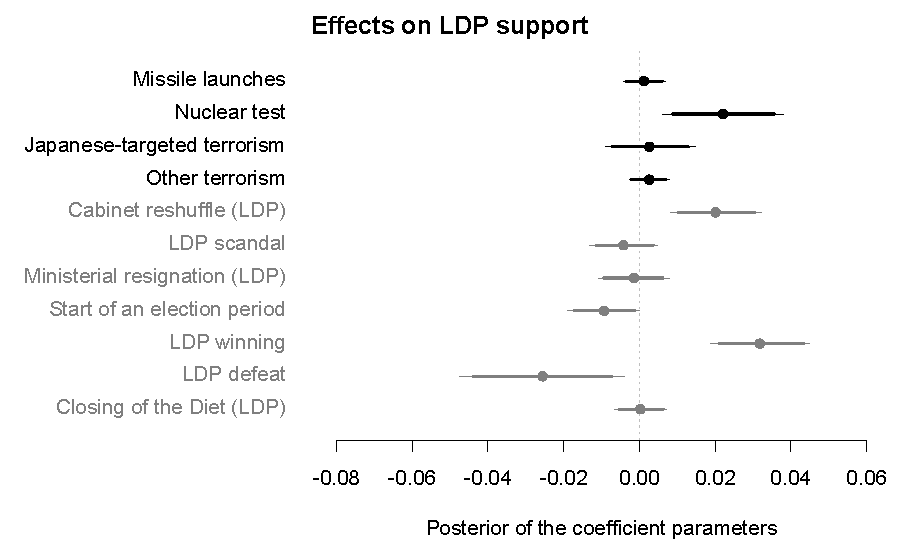
\includegraphics[scale=1]{Figure_POQ/average_effect_on_LDP_support.pdf}
\caption{Average Effects of Military Threat, Terrorism, and Other Control Variables on LDP Support Ratings}
\label{average_effect_on_LDP_support}
\end{minipage}
\begin{minipage}{\hsize}
\singlespacing
\small
\emph{Notes}: Dots represent point estimates, and thick and thin lines correspond to 90\% and 95\% CIs, respectively.
\end{minipage}
\end{figure}

The remainder of this section presents supplemental results. The bottom panel of Figure~\ref{approval_time_series} shows the weekly LDP support ratings estimated by Equation~\eqref{transition_model} in the main text. Figure~\ref{house_mode_design_LDP} and Table~\ref{miscellaneous_LDP} show the estimation results of miscellaneous parameters in the analysis of LDP support.

\begin{figure}[p]
\begin{minipage}{\hsize}
\centering
\singlespacing
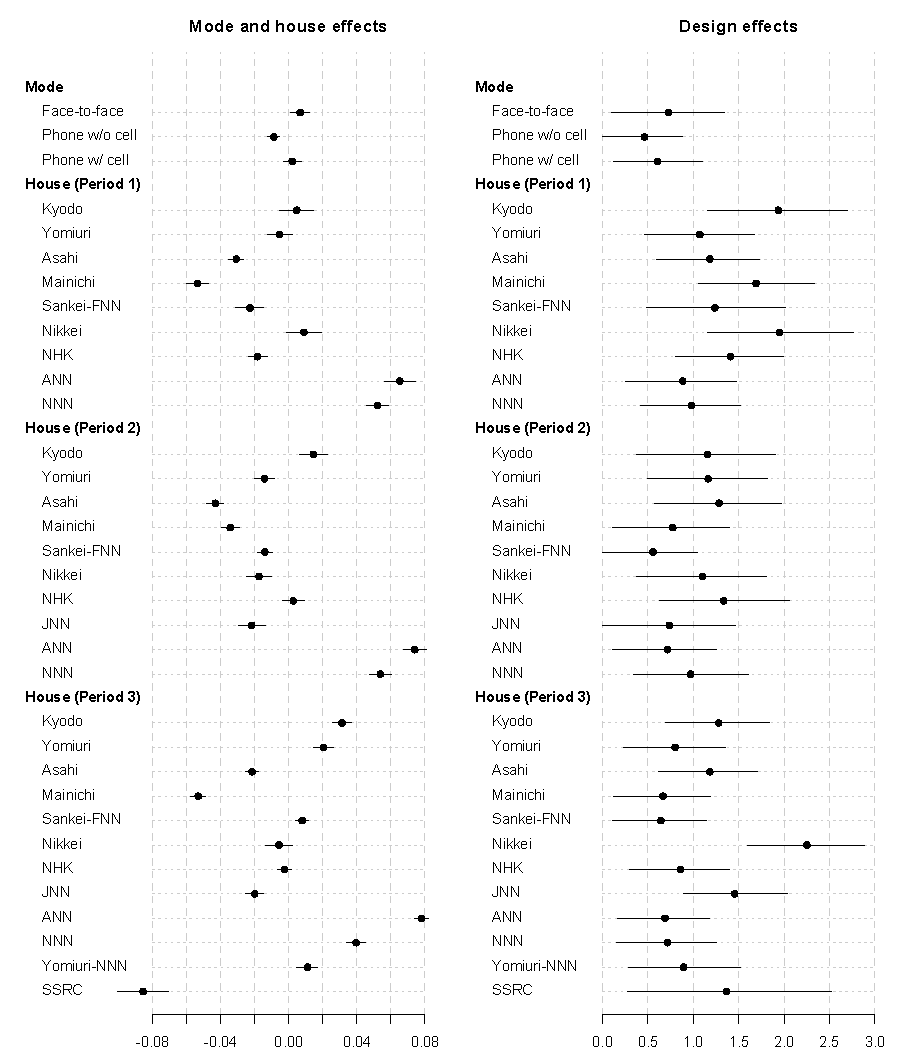
\includegraphics[scale=1]{Figure_POQ/miscellaneous_LDP_support.pdf}
\caption{Estimation Results of House, Mode, and Design Effects for LDP Support Ratings}
\label{house_mode_design_LDP}
\end{minipage}
\begin{minipage}{\hsize}
\singlespacing
\small
\emph{Notes}: Dots represent point estimates, and lines represent 95\% CIs.
\end{minipage}
\end{figure}

\begin{table}[h]
\centering
\small
\singlespacing
\caption{Estimation Results of Miscellaneous Parameters}
\label{miscellaneous_LDP}
\bigskip
\begin{tabular}{ld,}\toprule
 & \multicolumn{1}{c}{Point est.} & \multicolumn{1}{c}{95\% CI} \\\midrule
$\beta $ & 0.000 & [0.000,\: 0.000] \\
$\psi $ & 0.005 & [0.002,\: 0.009] \\
$\phi $ & 0.983 & [0.973,\: 0.993] \\
$\omega $ & 0.010 & [0.009,\: 0.011] \\\bottomrule
\end{tabular}
\end{table}

\clearpage
\subsection{Analysis of the Duration of the Effects}\label{app:subsec:duration}

Table~\ref{app:table_kappa_lambda_eta} presents estimates of $\bm{\kappa}$, $\bm{\lambda}$, and $\bm{\eta }$ in the transition model, which represent the duration of the rally effects on the LDP support, as shown in Equation~\eqref{transition_model_2} in the main text. The coefficients in $\bm{\kappa}$ are interpreted as the effects of events occurring on a Friday, meaning these events are close to weekend-conducted opinion polls. Our focus is on $\bm{\lambda}$, which indicates the duration of an event's effect. Negative (positive) $\bm{\lambda}$ values indicate that the rally effects attenuate (strengthen) over time after rally-inducing events. The results indicate that the coefficients of our main explanatory variables do not exhibit meaningful interactions with the temporal distance between events and polls. All parameters in $\bm{\lambda}$ include zero in their 95\% CIs.

\begin{table}[!ht]
\centering
\small
\singlespacing
\caption{Parameter Estimates of the Transition Model for LDP Support with Interaction Terms between Events and their Temporal Distance to Opinion Polls}
\label{app:table_kappa_lambda_eta}
\bigskip
\begin{tabular}{ld,}\toprule
 & \multicolumn{1}{c}{Point est.} & \multicolumn{1}{c}{95\% CI} \\\midrule
$\bm{\kappa}$ & &  \\
Missile launch  & 0.006 & [-0.009,\: 0.021] \\
Nuclear test & 0.010 & [-0.010,\: 0.041] \\
Japanese-targeted terrorism & 0.013 & [-0.016,\: 0.041] \\
Other terrorism & 0.000 & [-0.012,\: 0.012] \\
$\bm{\lambda}$ & & \\
Missile launch & -0.001 & [-0.004,\: 0.002] \\
\hspace{1em}$\times $ temporal distance & & \\
Nuclear test  & 0.003 & [-0.004,\: 0.010] \\
\hspace{1em}$\times $ temporal distance & &  \\
Japanese-targeted terrorism & -0.003 & [-0.009,\: 0.004] \\
\hspace{1em}$\times $ temporal distance  & & \\
Other terrorism & 0.001 & [-0.002,\: 0.003] \\
\hspace{1em}$\times $ temporal distance & & \\
$\bm{\eta}$ & & \\
Cabinet reshuffle & 0.020 & [0.008,\: 0.032] \\
Ministerial scandal & -0.004 & [-0.013,\: 0.005] \\
Ministerial resignation & -0.001 & [-0.010,\: 0.008] \\
Start of an election period & -0.009 & [-0.019,\: 0.000] \\
LDP victory & 0.031 & [0.018,\: 0.045] \\
LDP defeat & -0.026 & [-0.047,\: -0.003] \\
Closing of the Diet & 0.000 & [-0.006,\: 0.008] \\\bottomrule
\end{tabular}
\end{table}

\singlespacing
\subsection{Discussion about the Effect Heterogeneity between Cabinet Approval and LDP Support}\label{app:subsec:heterogeneity}
\doublespacing

The variations in effect sizes and their duration for military threats and terrorism can be attributed to different underlying mechanisms. On one hand, the rally effect of nuclear tests, which boosts approval for the cabinet and the LDP, is likely due to the activation of national identity among Japanese people and a shift in citizens' foreign policy preferences toward a more hawkish stance. Foreign policy and security issues are the primary dispute in post-war Japan: despite its constitution containing a pacifist clause, which proscribes the maintaining of armed forces, the Japan Self-Defense Forces are de facto military forces. Since the LDP's call for increasing Japanese military power is widely known, a perceived military threat seems likely to increase public support for the LDP. Because all six North Korean nuclear tests were conducted while the LDP was in power, we interpret the increase in cabinet approval ratings following each nuclear test reflects the increase in voter support for the LDP's aggressive foreign and security policies.

On the other hand, since terrorist attacks have short-lived effects on cabinet approval and no effect on LDP support, the threat of terrorism seems to cause temporary anxiety among citizens, in turn increasing support for the status quo. This interpretation corresponds with motivated social cognition theory \citep{Jost2003PsycholBull} and theory on the relationship between threat and authoritarianism \citep{Doty1991JPSP}. Our finding that the rally effect of terrorist attacks lasts only a few days implies that psychological change in anxiety and status quo preference might be very small and temporary. However, an alternative perspective is that minor events seemingly unrelated to particular individuals could psychologically influence their political orientation.

\clearpage
\bibliographystyle{apsr2}
\bibliography{bib_rally_round_the_flag,Rally,rally_tomoya}
\end{document}